\section{Paketverlust erkennen}
\label{sec:Paketverlust erkennen}

\subsection{Datenstruktur für die \esp Verbindungen}
Für die Datenstruktur in GO musste ein Ersatz für bekannte Datenstrukturen wie Hashmap und Liste gefunden werden. Die Hashmap wurde in Go mit dem Typ "map" umgesetzt. Als Ersatz für eine Liste werden "Slices" eingesetzt. Dieser Typ ähnelt sehr einem Array, kann aber beliebig wachsen und schrumpfen und sind dennoch sehr Ressourcen schonend.\\

Die Datenstruktur besteht grundsätzlich aus einer Hashmap zum speichern der Verlorenen Pakete für jede VPN-Verbindung.
Eine VPN-Verbindung wird identifiziert mit den Werten für \acs{SPI} der Source- sowie der Destinationadresse.\\
Als Value werden grundsätzlich zwei Listen für die Lost und MaybeLost Pakete benötigt.\\ 
Wobei MaybeLost für die Sequenznummern der Pakete die als fehlend erkannt wurden aber noch innerhalb des ESP-Window liegen gedacht ist.\\
Lost hingegen ist für Sequenznummern der Pakete die als Verloren erkannt wurden oder zu spät angekommen sind.\\
Zusätzlich wird noch ein Wert für den aktuellen Head gespeichert.\\
Durch diese Aufteilung, können Pakete beziehungsweise deren Sequenznummern sehr effektiv verwaltet werden.

\begin{figure}[H]
    \begin{center}
        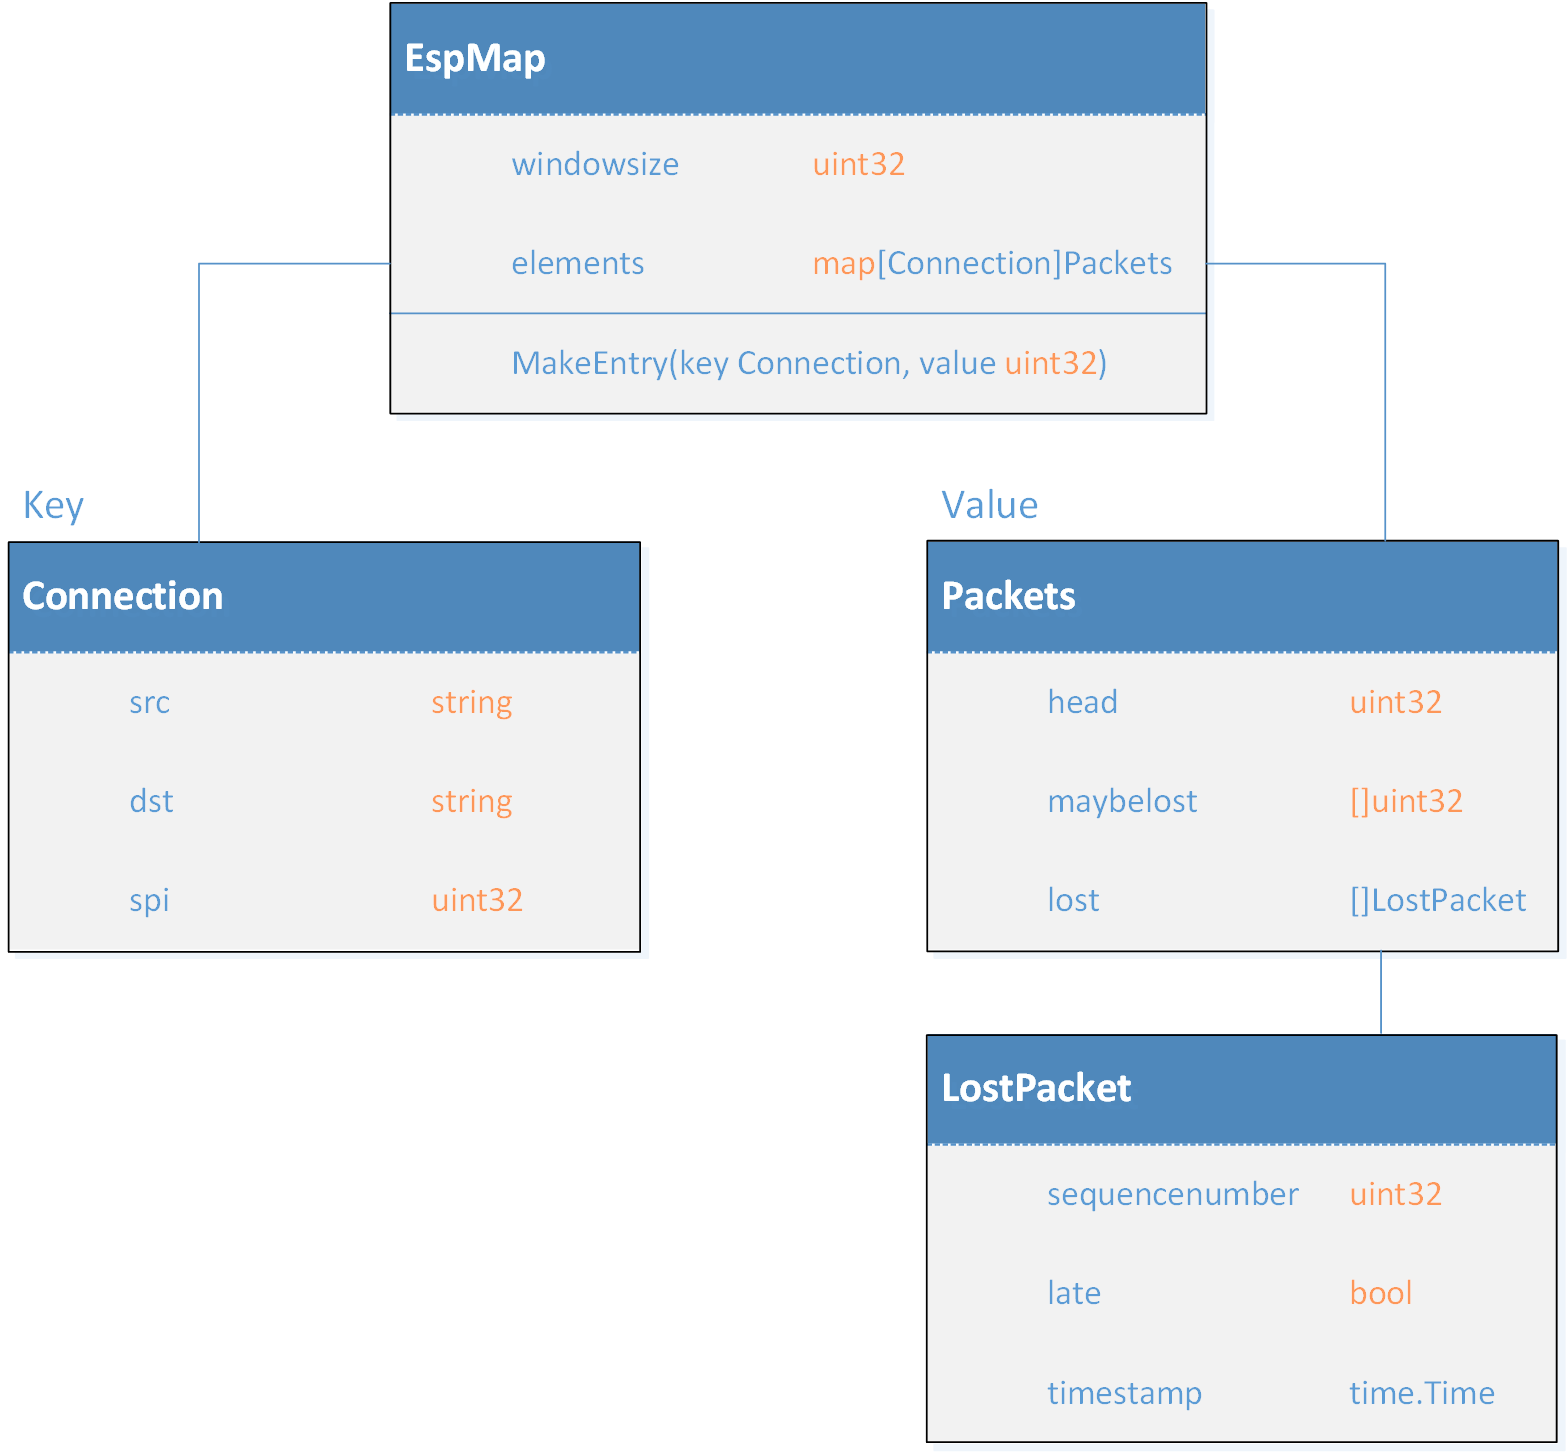
\includegraphics[trim=1 0 0 0,clip,width=\textwidth]{start/img/Datenstruktur.png}
    \end{center}
    \caption{Datenstruktur zur Feststellung des Paketverlusts}
\end{figure}

\subsection{Erkennung des Paketverlusts}
Die Paketverluste werden mit folgendem Algorithmus festgestellt. 
Vereinfachte Darstellung des Algorithmus in Pseudocode:\\
\textbf{Neues Packet Verarbeiten}
\begin{lstlisting}[language=go]
If(neuesPaket > Head){
	If(neuesPaket != Head + 1){
		Pakete von Head bis neuesPaket in MaybeLost speichern
	}
	Head = neuesPaket
	CheckLost()
}else{
	If(Head-WindowSize<neuesPaket){
		Packet aus MaybeLost entfernen
	}
	else{
		Flag setzen fuer zu spaet angekommen
	}
}
\end{lstlisting}

\textbf{CheckLost}
\begin{lstlisting}[language=go]
for(MaybeLost){
	if(Head-WindowSize >= MaybeLostEintrag){
		Paket in Lost Speichern
		Paket aus MaybeLost entfernen
}
CheckLog()
\end{lstlisting}

\textbf{CheckLog}
\begin{lstlisting}[language=go]
for(LostPackets){
	if(in Time Window){
		counter++
	}
}
if(counter>=AlertCounter){
	Alert()
}
\end{lstlisting}


\section{ Meldungsaufbau}

\noindent Die Bedingungen für das Auslösen eines Alerts können im Configfile festgelegt werden. Es können der Zeitraum und die Anzahl Pakete definiert werden. Falls innerhalb dieses definierten Zeitraums die Anzahl an verlorenen Paketen überschritten wird, wird ein Alert ausgelöst.

\noindent Der Alert besitzt folgende Form:

\begin{table}[H]
\begin{tabularx}{\textwidth}{l|l|>{\raggedright\arraybackslash}X} 
\textbf{Severity} & \textbf{Programm} & \textbf{Meldung}\\ 
\hline
1 & IPsecDiagTool & Too much LostPackets in Connection: (SPI: \dots ,SRC:\dots ,DST\dots
\end{tabularx}
\caption{Aufbau der Syslog-Nachricht}
\end{table}

\noindent So kann gleich anhand der Meldung erkannt werden, um welche Verbindung es sich handelt und die notwendigen Schritte für eine Korrektur vorgenommen werden.

\noindent Damit es nicht zu einer Flut von Benachrichtigungen mit dem gleichen Inhalt und den gleichen Paketen kommt, wurde ein Timer von 10 Sekunden eingeführt.

\section{ Logging Package}

\noindent Das Logging wurde in einem separaten Package umgesetzt und stellt Methoden für das Logging zur Verfügung. Die Package kapselt die benötigte Funktionalität, die von \code{log/syslog} benötigt wird.

\noindent Das Package wird vor Verwendung der Logging Funktionalität durch InitLogger initialisiert. Dabei werden die Werte für Zeitfenster, Anzahl Packete und Syslogserver gesetzt. Danach können die Benachrichtigungen mit AlertLog und InfoLog erstellt werden.

\section{ Benachrichtigung mit Datei}

\noindent Gleichzeitig mit dem Syslogeintrag wird eine CSV Datei erstellt. Die Datei beinhaltet detaillierte Informationen um welche verlorenen Pakete es sich handelt und mit welchem Abstand ein Verlust detektiert wurde. Ausserdem gibt es Informationen, ob ein Paket möglicherweise zu spät eingetroffen ist (also ausserhalb des Windows für die Sequenznummern). Falls dieses Problem vermehrt eintritt, könnte ein Erhöhen der Window-Size nötig sein.

\noindent Die Datei wurde so angepasst, dass sie mit Microsoft Excel oder ähnlichen Programmen problemlos gelesen und weiter verarbeitet werden kann.

\noindent Beispiel einer Datei

\begin{figure}[H]
    \begin{center}
        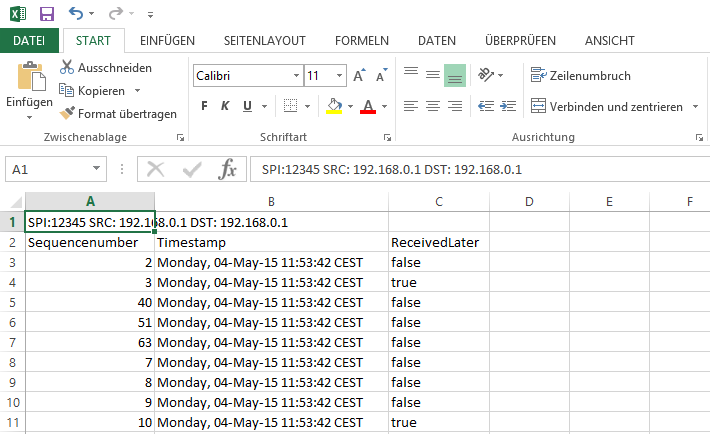
\includegraphics[trim=1 0 0 0,clip,width=\textwidth]{start/img/Datei.png}
    \end{center}
    \caption{Beispiel einer generierten CSV Datei}
\end{figure}